\begin{problem}{/images/problems/24_dices.jpg}{Boxes and Dice}We have 6 boxes numbered from 1 to 6. Each box has a label on it originally equal to 1 for all boxes (notice that the numbers and labels are two separate concepts). Each time, we roll two dice. Let the number of the first die be $x$ and the number of the second die be $y$. We change the label of box $x$ to $y$.

On average, how many times do we need to repeat this until the labels of the boxes are equal to their numbers?\\[0.2cm]

\textbf{Supplementary question}: on average, how many times do we repeat this process until the labels of all 6 boxes are distinct?\\[0.2cm]

Link to the problem on Twitter:  \url{https://twitter.com/Riazi_Cafe/status/1690240896535789568}\end{problem}
\begin{solution}
The correct answer for the problem is 58501.2. Also, the answer to the supplementary problem is equal to 90.36.\\[0.2cm]

\textbf{Explanation of the first part}: At any moment in time, the only factor that determines how many steps are required on average for the labels on the boxes to be desirable is how many labels written on the boxes are desired? At first, because all the labels are equal to one, this amount is equal to 1. Because  only the label of the first box desired.

Based on this, the problem can be modeled as a graph:
We have a graph with 7 vertices, where vertex number $i$ represents all states in which $i$ boxes are desirable. At first, there is a token on vertex number  1. In each step, this token moves to one of the vertices of the graph (including the current vertex) based on certain probabilities. On average, how many steps does it take for the token to reach vertex number 6?

In the figure, you can see the probability of moving from each vertex to other vertices:

\begin{center}
	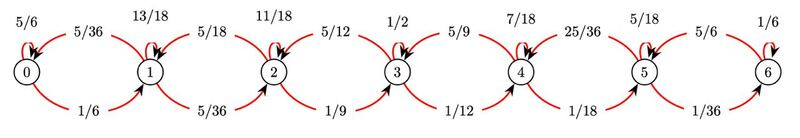
\includegraphics{/images/problems/24_diagram1.png}
\end{center}

Problems like this are called Markov chain and can be solved as a system of equations. In this system, for each vertex $i$, there is a variable $v_i$ that shows the answer of the problem when starting with the token placed on that node.

The system of equations for our problem is as follows:

$$
\begin{aligned}
&v_0 = 1 + \frac{5}{6}v_0 + \frac{1}{6}v_1 \\
&v_1 = 1 + \frac{5}{36}v_0 + \frac{13}{18}v_1 + \frac{5}{36}v_2 \\
&v_2 = 1 + \frac{5}{18}v_1 + \frac{11}{18}v_2 + \frac{1}{9}v_3 \\
&v_3 = 1 + \frac{5}{12}v_2 + \frac{1}{2}v_3 + \frac{1}{12}v_4 \\
&v_4 = 1 + \frac{5}{9}v_3 + \frac{7}{18}v_4 + \frac{1}{18}v_5 \\
&v_5 = 1 + \frac{25}{36}v_4 + \frac{5}{18}v_5 + \frac{1}{36}v_6 \\
&v_6 = 0
\end{aligned}
$$

The solution of this equation system is as follows:

$$
\begin{aligned}
&v_0 = 58507.2 \\
&v_1 = 58501.2 \\
&v_2 = 58488 \\
&v_3 = 58446 \\
&v_4 = 58224 \\
&v_5 = 55986 \\
&v_6 = 0
\end{aligned}
$$

Because we start from vertex number 1, then the answer to the problem is equal to 58501.2.

\textbf{Explanation of the second part}: With the same method, we can also solve the second problem. However, the  graph is a  bigger, and thus, solving the questions requires programming.

In this case, the factor that determines how many steps are left on average is the following:
``what is the count of each of the distinct labels we have on the boxes?''\\[0.2cm]
Notice that the labels themselves and their orders are not important and only the count of the groups is important.
For example, if 1 3 1 5 5 2 are written on the boxes, the corresponding state is $(2,2,1,1)$ because 4 distinct labels are written on the boxes, two of which are equal to 1, two of which are equal to 5, and there is a single  $2$ and a single $3$ among them.
Also, if 6 6 1 2 4 4 were written on the boxes, the corresponding state would still be  $(2,2,1,1)$ even though the labels are different from the previous example. However, the size of the groups of distinct labels is the same as the previous example.

At first, the labels written on the 6 boxes are the same, therefore we start from state (6). The goal is to go to the state $(1,1,1,1,1,1)$ which represents that case that all 6 labels are distinct.

We define these different states as follows:

$$
\begin{aligned}
v_0&=(6)\\
v_1&=(5,1)\\
v_2&=(4,2)\\
v_3&=(3,3)\\
v_4&=(4,1,1)\\
v_5&=(3,2,1)\\
v_6&=(2,2,2)\\
v_7&=(3,1,1,1)\\
v_8&=(2,2,1,1)\\
v_9&=(2,1,1,1,1)\\
v_{10}&=(1,1,1,1,1,1)
\end{aligned}
$$

Below are the graph of the problem and the system of equations for the answer:

\begin{center}
	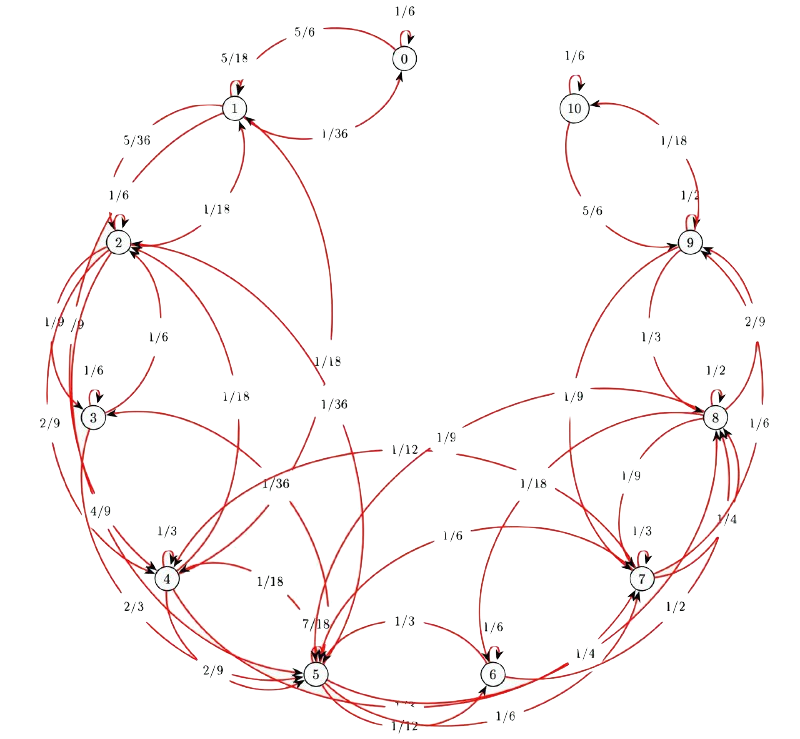
\includegraphics[width=12cm]{/images/problems/24_diagram2.png}
\end{center}


$$
\begin{aligned}
&v_0 = 1 + \frac{1}{6}v_0 + \frac{5}{6}v_1 \\
&v_1 = 1 + \frac{1}{36}v_0 + \frac{5}{18}v_1 + \frac{5}{36}v_2 + \frac{5}{9}v_4 \\
&v_2 = 1 + \frac{1}{18}v_1 + \frac{1}{6}v_2 + \frac{1}{9}v_3 + \frac{2}{9}v_4 + \frac{4}{ 9}v_5 \\
&v_3 = 1 + \frac{1}{6}v_2 + \frac{1}{6}v_3 + \frac{2}{3}v_5 \\
&v_4 = 1 + \frac{1}{18}v_1 + \frac{1}{18}v_2 + \frac{1}{3}v_4 + \frac{2}{9}v_5 + \frac{1}{ 3}v_7 \\
&v_5 = 1 + \frac{1}{36}v_2 + \frac{1}{36}v_3 + \frac{1}{18}v_4 + \frac{7}{18}v_5 + \frac{1}{ 12}v_6 + \frac{1}{6}v_7 + \frac{1}{4}v_8 \\
&v_6 = 1 + \frac{1}{3}v_5 + \frac{1}{6}v_6 + \frac{1}{2}v_8 \\
&v_7 = 1 + \frac{1}{12}v_4 + \frac{1}{6}v_5 + \frac{1}{3}v_7 + \frac{1}{4}v_8 + \frac{1}{ 6}v_9 \\
&v_8 = 1 + \frac{1}{9}v_5 + \frac{1}{18}v_6 + \frac{1}{9}v_7 + \frac{1}{2}v_8 + \frac{2}{ 9}v_9 \\
&v_9 = 1 + \frac{1}{9}v_7 + \frac{1}{3}v_8 + \frac{1}{2}v_9 + \frac{1}{18}v_{10} \\
&v_{10} = 0
\end{aligned}
$$

The answer to the above system of equation is equal to:

$$
\begin{aligned}
v_0 &= 90.36 \\
v_1 &= 89.16 \\
v_2 &= 88.44 \\
v_3 &= 88.2 \\
v_4 &= 87.48 \\
v_5 &= 86.64 \\
v_6 &= 86.04 \\
v_7 &= 84.6 \\
v_8 &= 83.64 \\
v_9 &= 76.56 \\
v_{10} &= 0
\end{aligned}
$$

which means the average number of steps is equal to 90.36 for the second part.



\end{solution}
